\documentclass[a4paper, 11 pt]{article}

\usepackage[latin1]{inputenc}
\usepackage[english]{babel}
\usepackage{indentfirst}
\usepackage{graphicx}
\usepackage{subfigure}
\usepackage{mathtools}
\usepackage[retainorgcmds]{IEEEtrantools}
\usepackage{multirow}
\usepackage{array}
\usepackage{mhchem}
\usepackage{booktabs}
%\usepackage{psfrag}
\usepackage[hypcap=true]{caption}
\usepackage[bookmarks=true,hyperfootnotes=false]{hyperref}
\hypersetup{
	colorlinks=true,
	linkcolor=red,
	anchorcolor=red,
	citecolor=red,
	urlcolor=red,
	%linktocpage=true
	pdftitle={THGEM characterization},
	pdfauthor={I. Ciraldo, G.A. Brischetto}
}

\title{\bf {\huge THGEM characterization} }
\author{Dott. D. Torresi, I. Ciraldo, G.A. Brischetto}
\date{16 Dicembre 2019}

\begin{document}

\maketitle

\section{Introduction}

In view of the MAGNEX Focal Plane Detector (FPD) upgrade it is necessary to test the Thick Gas Electron Multipliers (THGEMs).
This new technology will substitute the present tracker, based on proportional wires.
It guarantees to cope with rate of the order of MHz/$\mbox{mm}^2$.
The aim of these tests was to study the THGEM response varying the induction, the THGEM and the drift tensions. 
In December 2019 two prototypes of THGEM were characterized. Both prototypes are multiple THGEM composed by three layers of GEM, but they show different hole pattern for the multiplication.


%Due parole sull'obiettivo dei test, caratterizzazione delle THGEM e del prototipo, focalizzandoci sulle risposte del sistema variando le THGEM

%Descrivere i due tipi di THGEM: foto, schemi, differenze, tabella FULL THGEM vs. ROW THGEM (indicando pitch, dimensione del foro e rim, spessore totale e spessore della metallizzazione (copper plating) )


%Micro patterned gas detector


\section{Experimental setup}

In these tests, two kinds of THGEM were employed: in the first one, referred to as FULL THGEM (Figure~\ref{fig:full_thgem}), the holes are uniformly distributed over the active surface; in the second one, called ROW THGEM (Figure~\ref{fig:row_thgem}), the holes are arranged in five rows.
In the FULL THGEM there are 143 rows of holes in horizontal and in vertical direction (Figure~\ref{fig:full_thgem_holes}), giving a total of 20449 holes.
In the ROW THGEM (Figure~\ref{fig:row_thgem_holes}) for each of the five rows there are 143 holes.
The main characteristics of the two prototypes are shown in Table~\ref{tab:thgem}.
The two THGEMs have the same dimensions: 107$\times$107~$\mbox{mm}^2$.

\begin{figure}
	\centering
		\subfigure[]{\label{fig:full_thgem}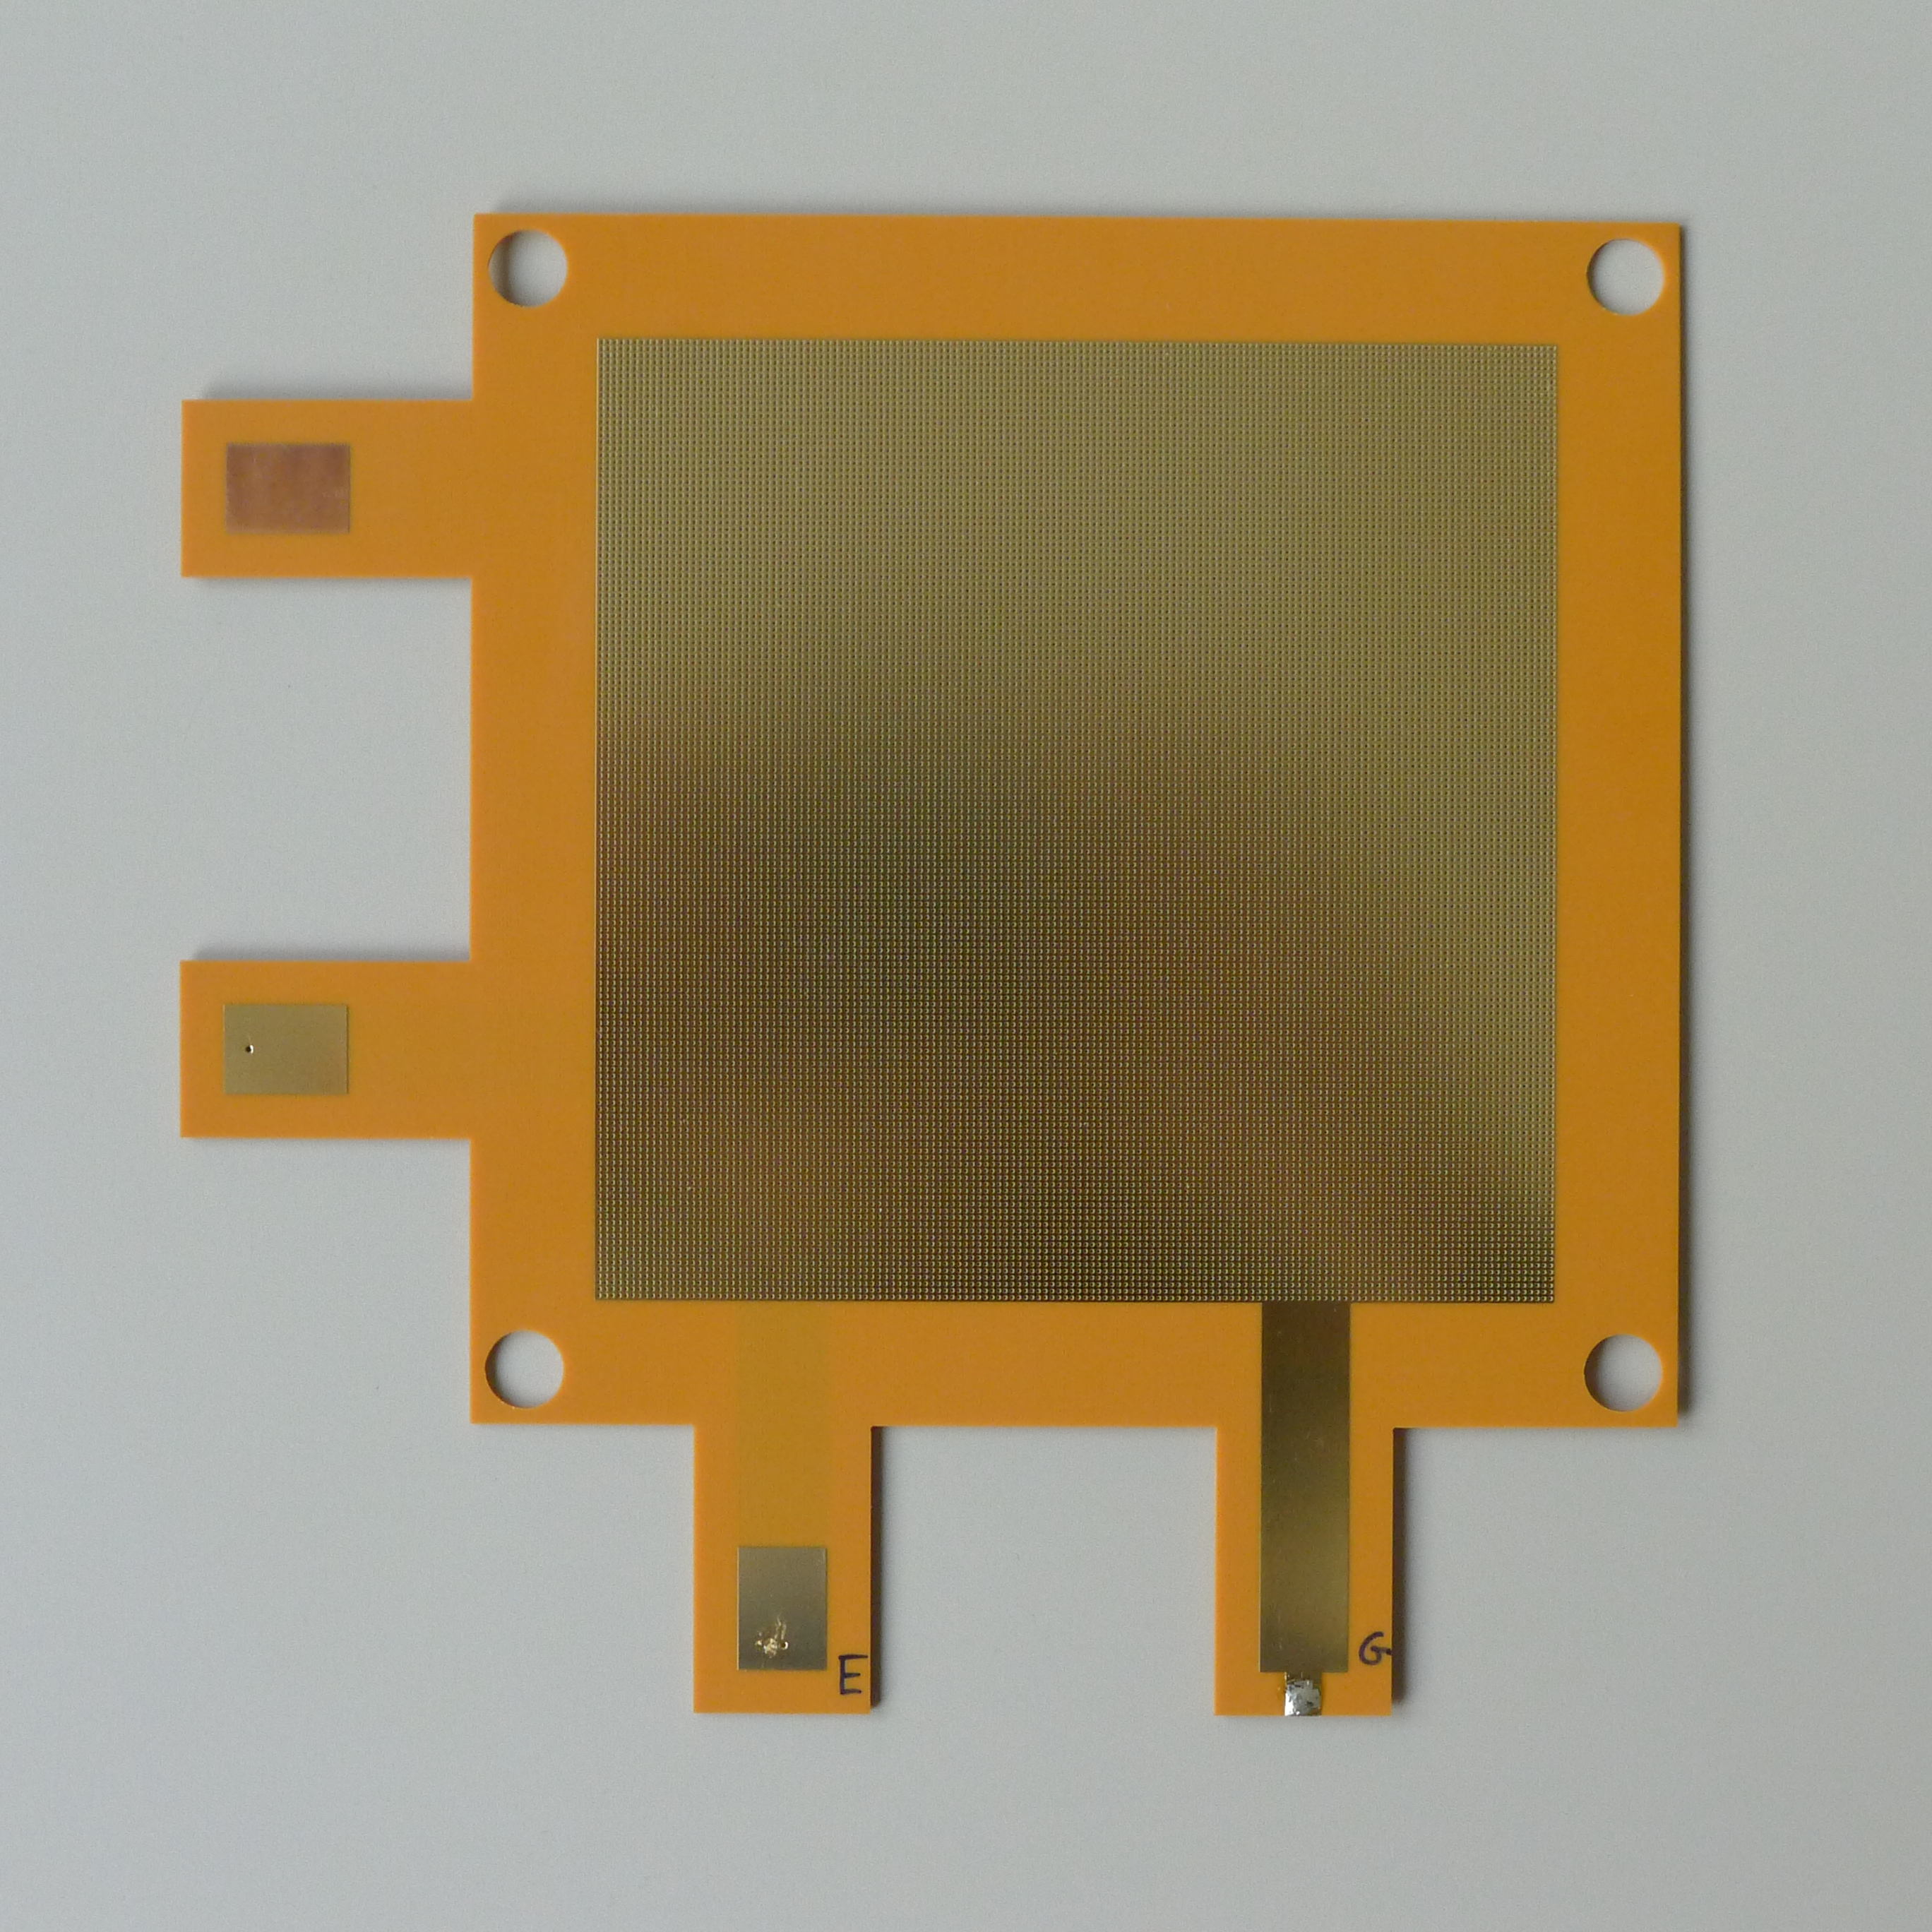
\includegraphics[width=0.45\textwidth]{Immagini/full_thgem.JPG}}
		\hspace{5pt}
		\subfigure[]{\label{fig:full_thgem_holes}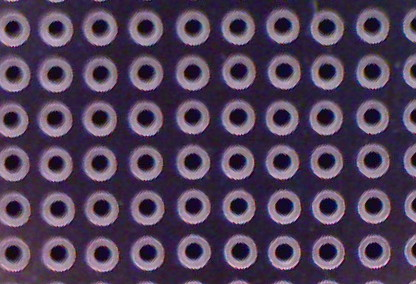
\includegraphics[width=0.45\textwidth]{Immagini/full_thgem_holes.JPG}}
	\caption{In (a) the FULL THGEM prototype, in (b) its hole pattern.}
	\label{fig:full_thgem_complessiva}		
\end{figure}

\begin{figure}
	\centering
	\subfigure[]{\label{fig:row_thgem}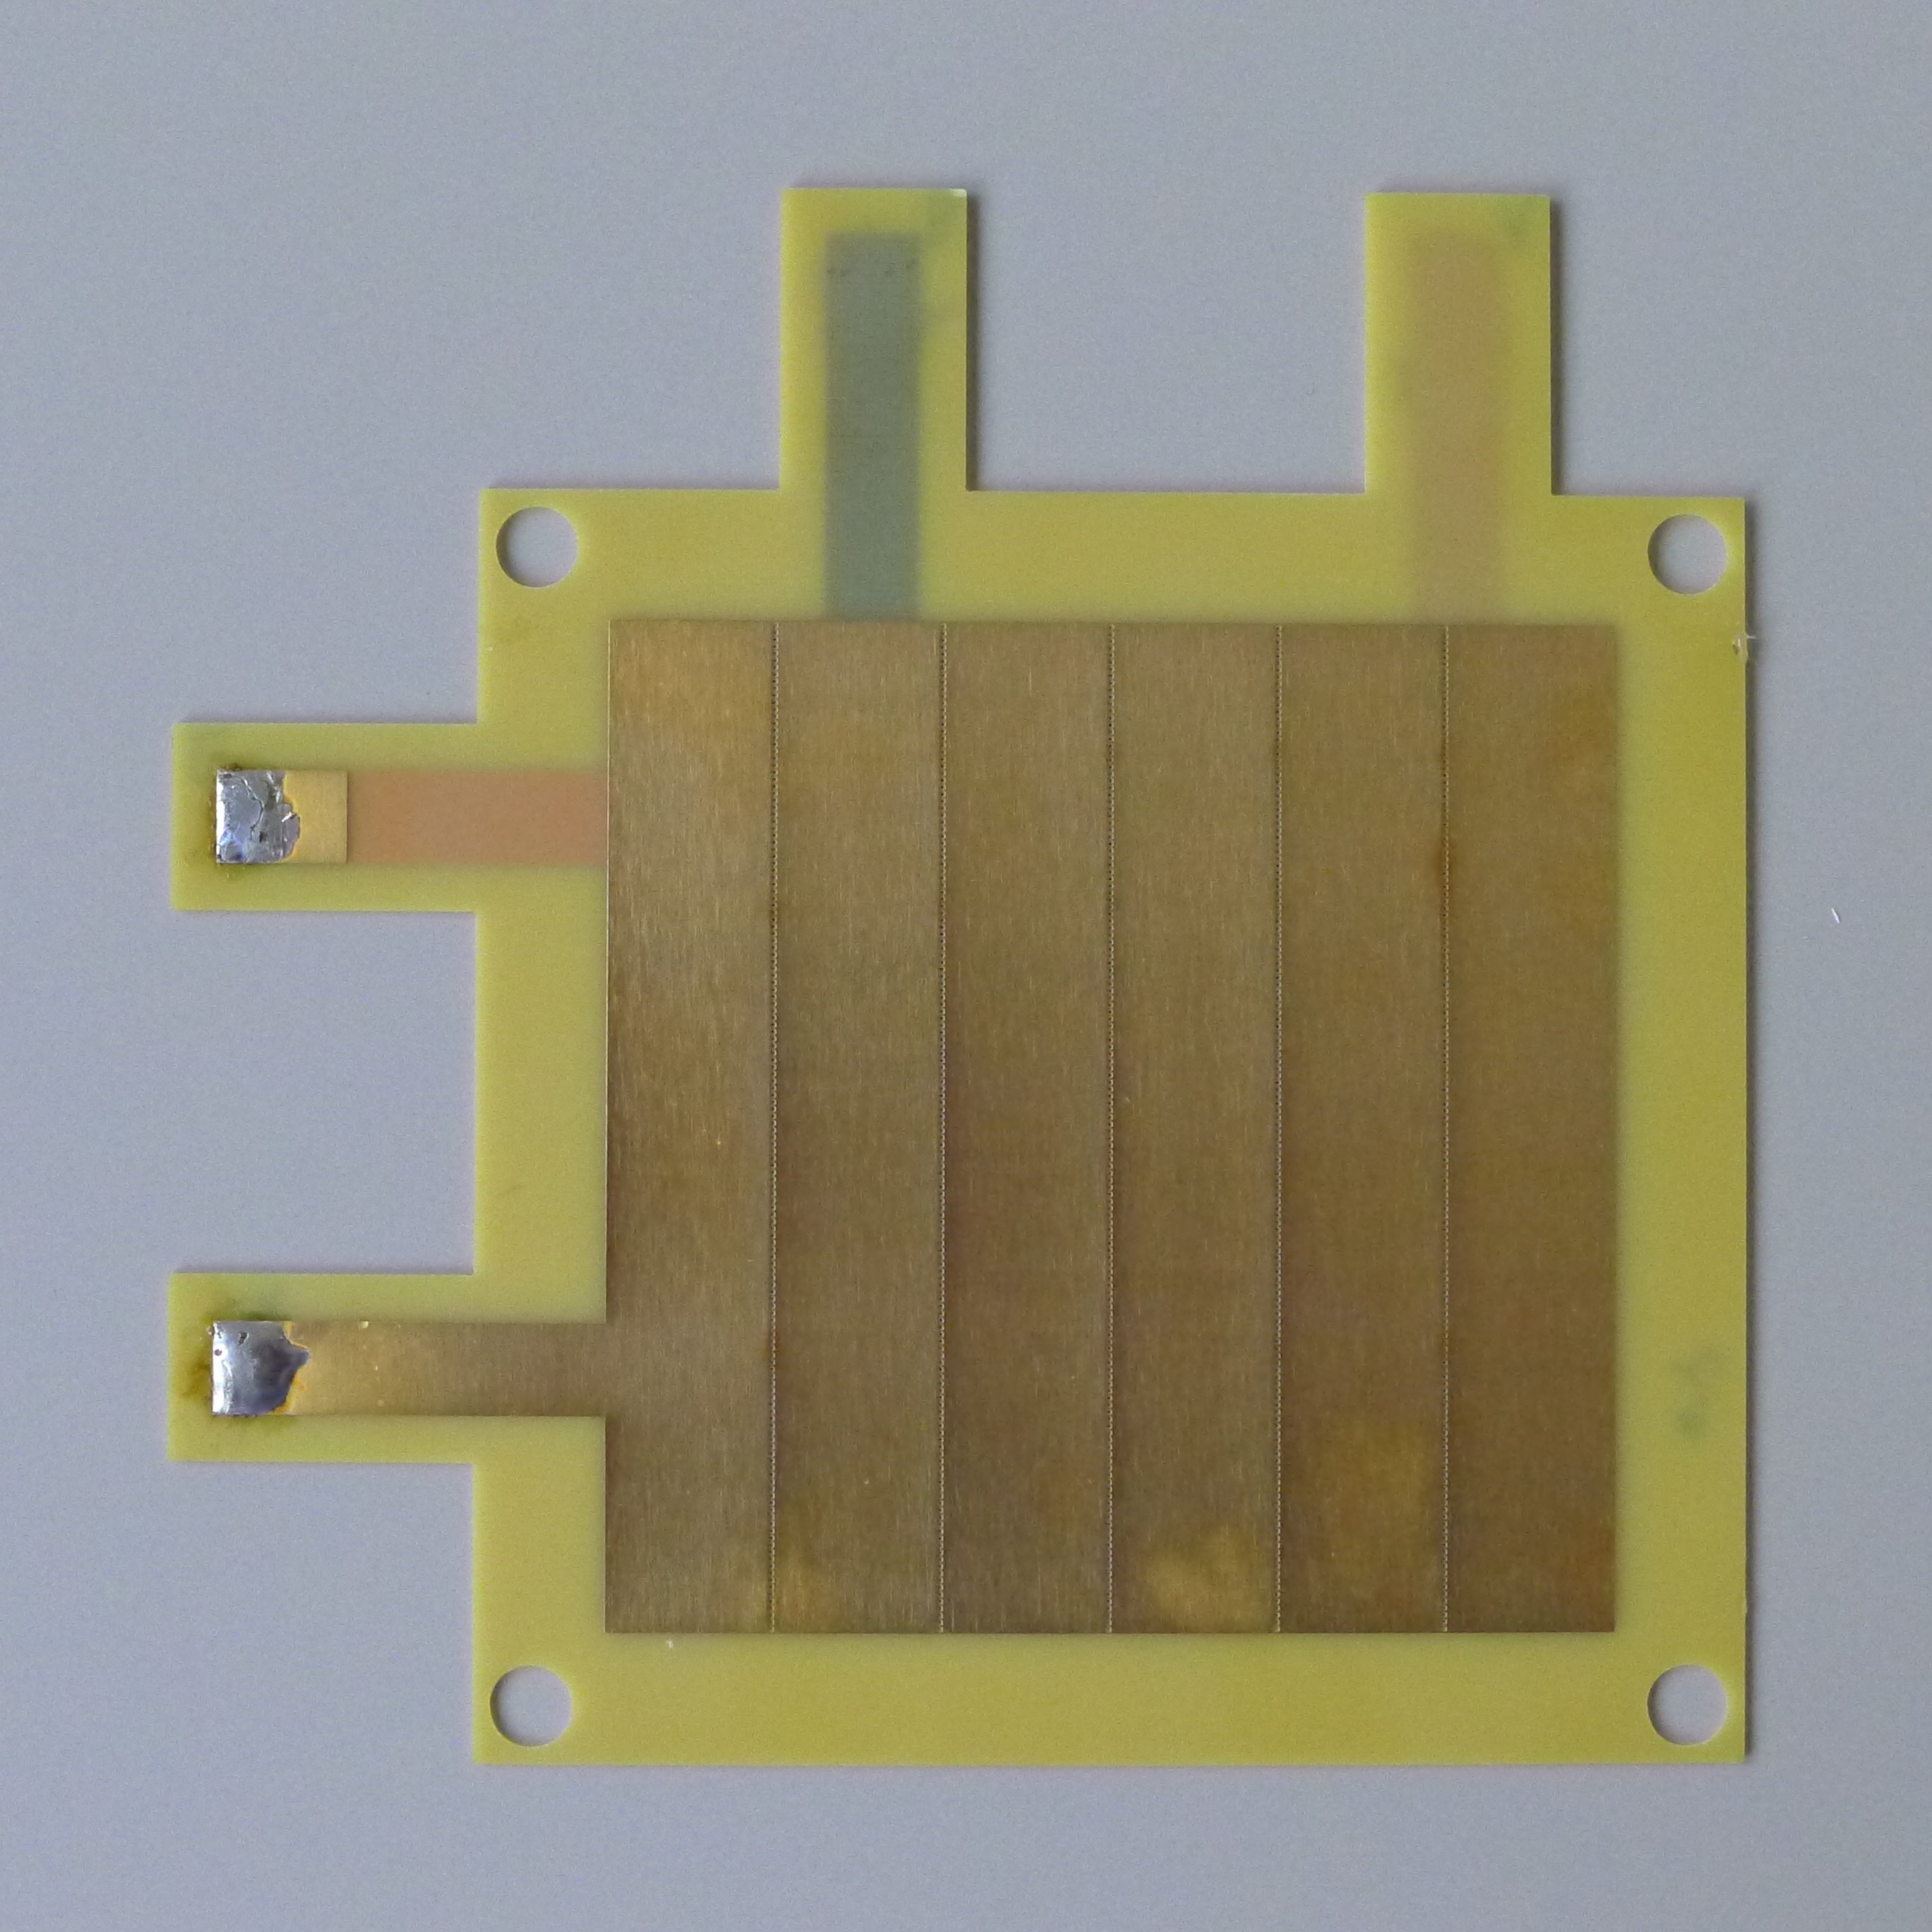
\includegraphics[width=0.45\textwidth]{Immagini/row_thgem.JPG}}
	\hspace{5pt}
	\subfigure[]{\label{fig:row_thgem_holes}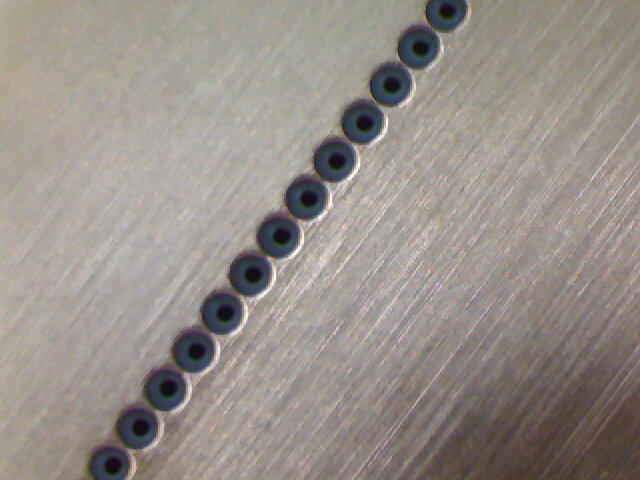
\includegraphics[width=0.45\textwidth]{Immagini/row_thgem_holes.JPG}}
	\caption{In (a) the ROW THGEM prototype, in (b) its hole pattern.}
	\label{fig:row_thgem_complessiva}		
\end{figure}

\begin{table} [b!]
	\begin{center}
		\renewcommand{\arraystretch}{1.2}
		\begin{tabular} {ccccc}
			Substrate &  Finish board   &  Hole diameter & Rim size  & Hole spacing \\
			material  &  thickness (mm) &      (mm)      &   (mm)    &   (mm)       \\
			
			\toprule[0.1em]
			%\hline
			Ceramic SD103K &  1.4 $\pm$ 0.1 & 0.30 $\pm$ 0.05 & 0.1 & 0.75 \\
			PCB 		   &  1.28 		 & 0.280		  & 0.2 & 0.75 \\
			
			\bottomrule[0.1em]
		\end{tabular}
	\end{center}
	\caption{The main characteristics of the two type of THGEM tested.} \label{tab:thgem}
\end{table}

The experimental apparatus used in the tests is composed by a gas chamber with inside the tracker prototype, an alpha source and a shutter. The shutter is used to allow or prevent alpha particles from arriving to the tracker. To supply the required voltages a CAEN system is employed. This system can be used also for measuring Anode, THGEM and Cathode currents as shown in Figure~\ref{fig:schema_canali}. The same currents were measured with better accuracy with the PICO system. PICO is a pico-amperometer and the lowest current measurable is.

\begin{figure}
	\centering
	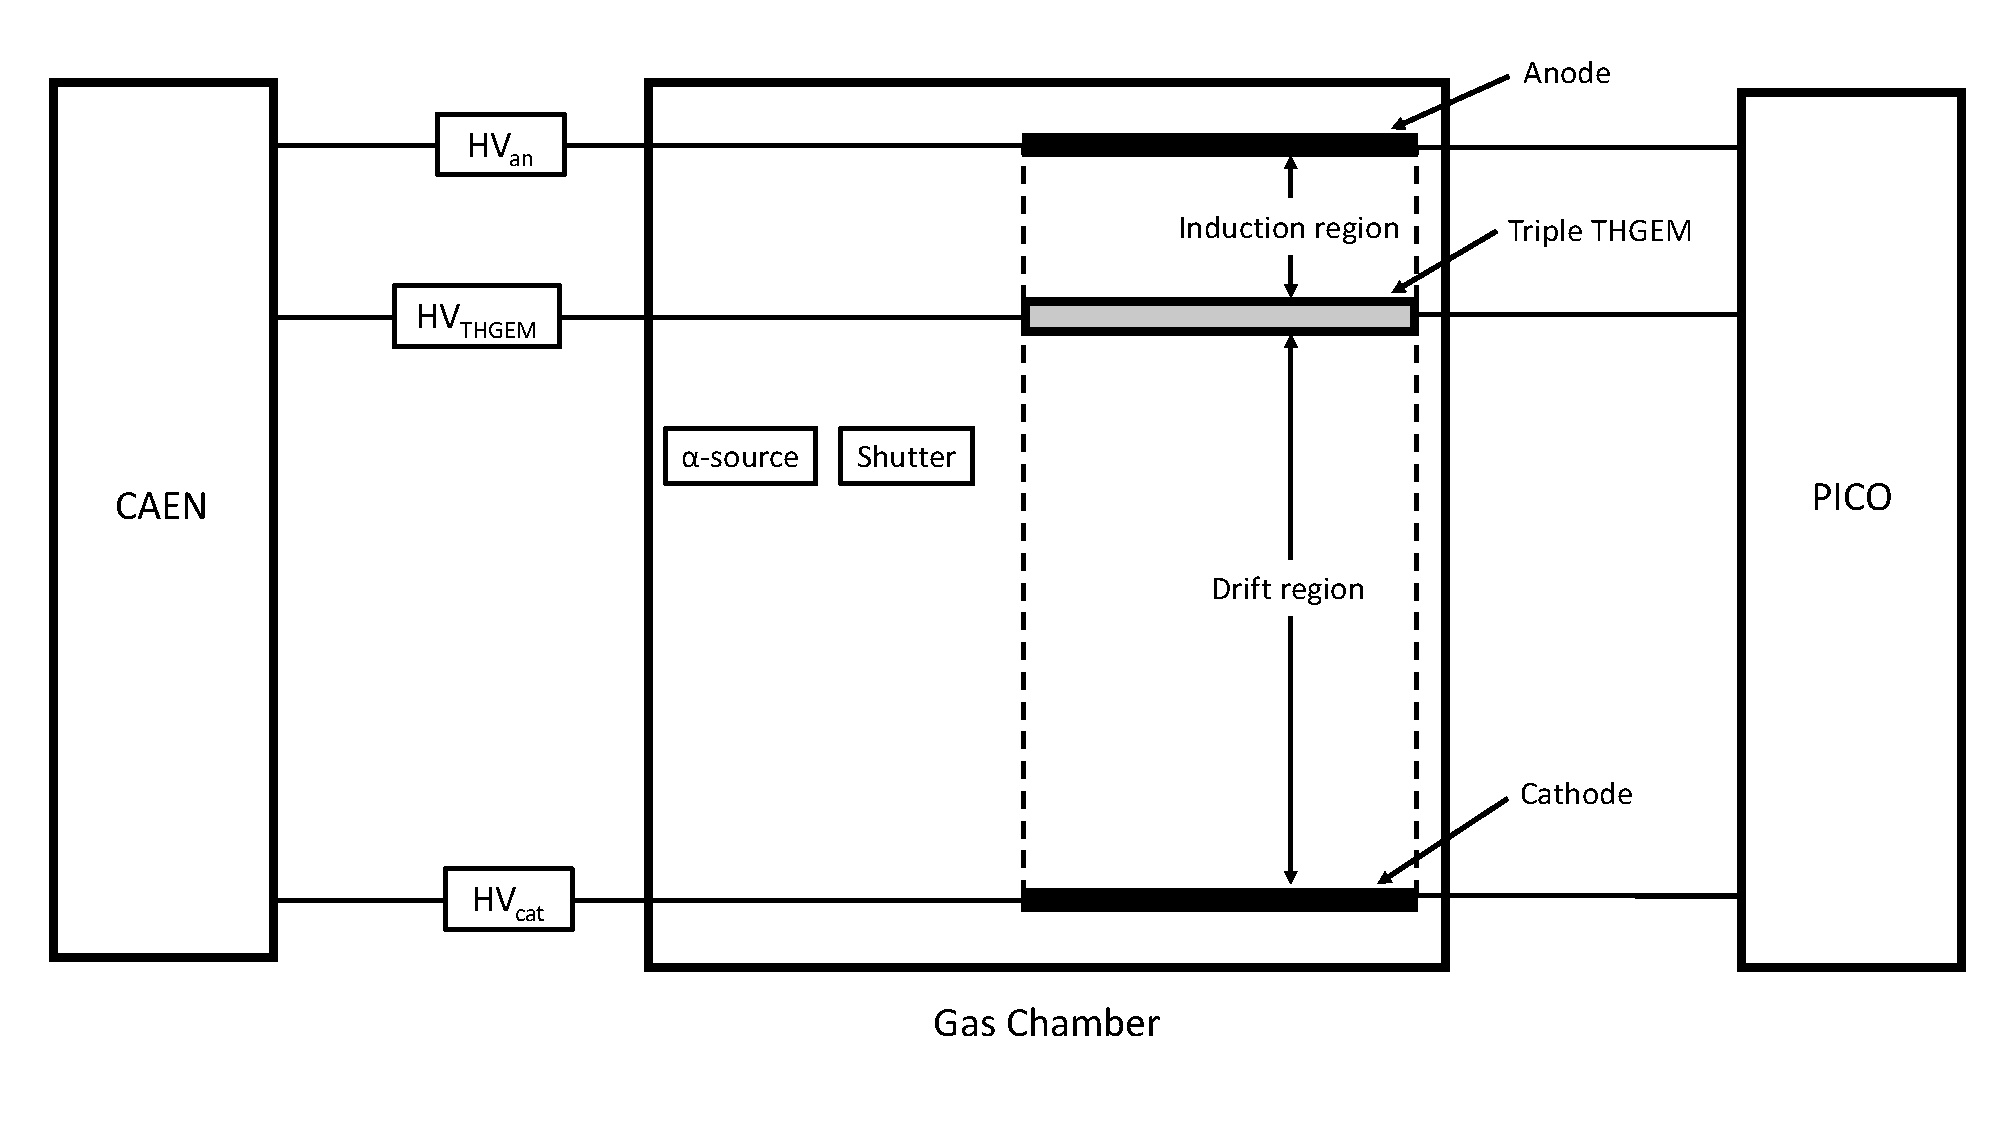
\includegraphics[width=0.8\textwidth]{Immagini/schema_apparato.pdf}
	\caption{The experimental set-up.}
	\label{fig:schema_apparato}
\end{figure}

\begin{figure}
	\centering
	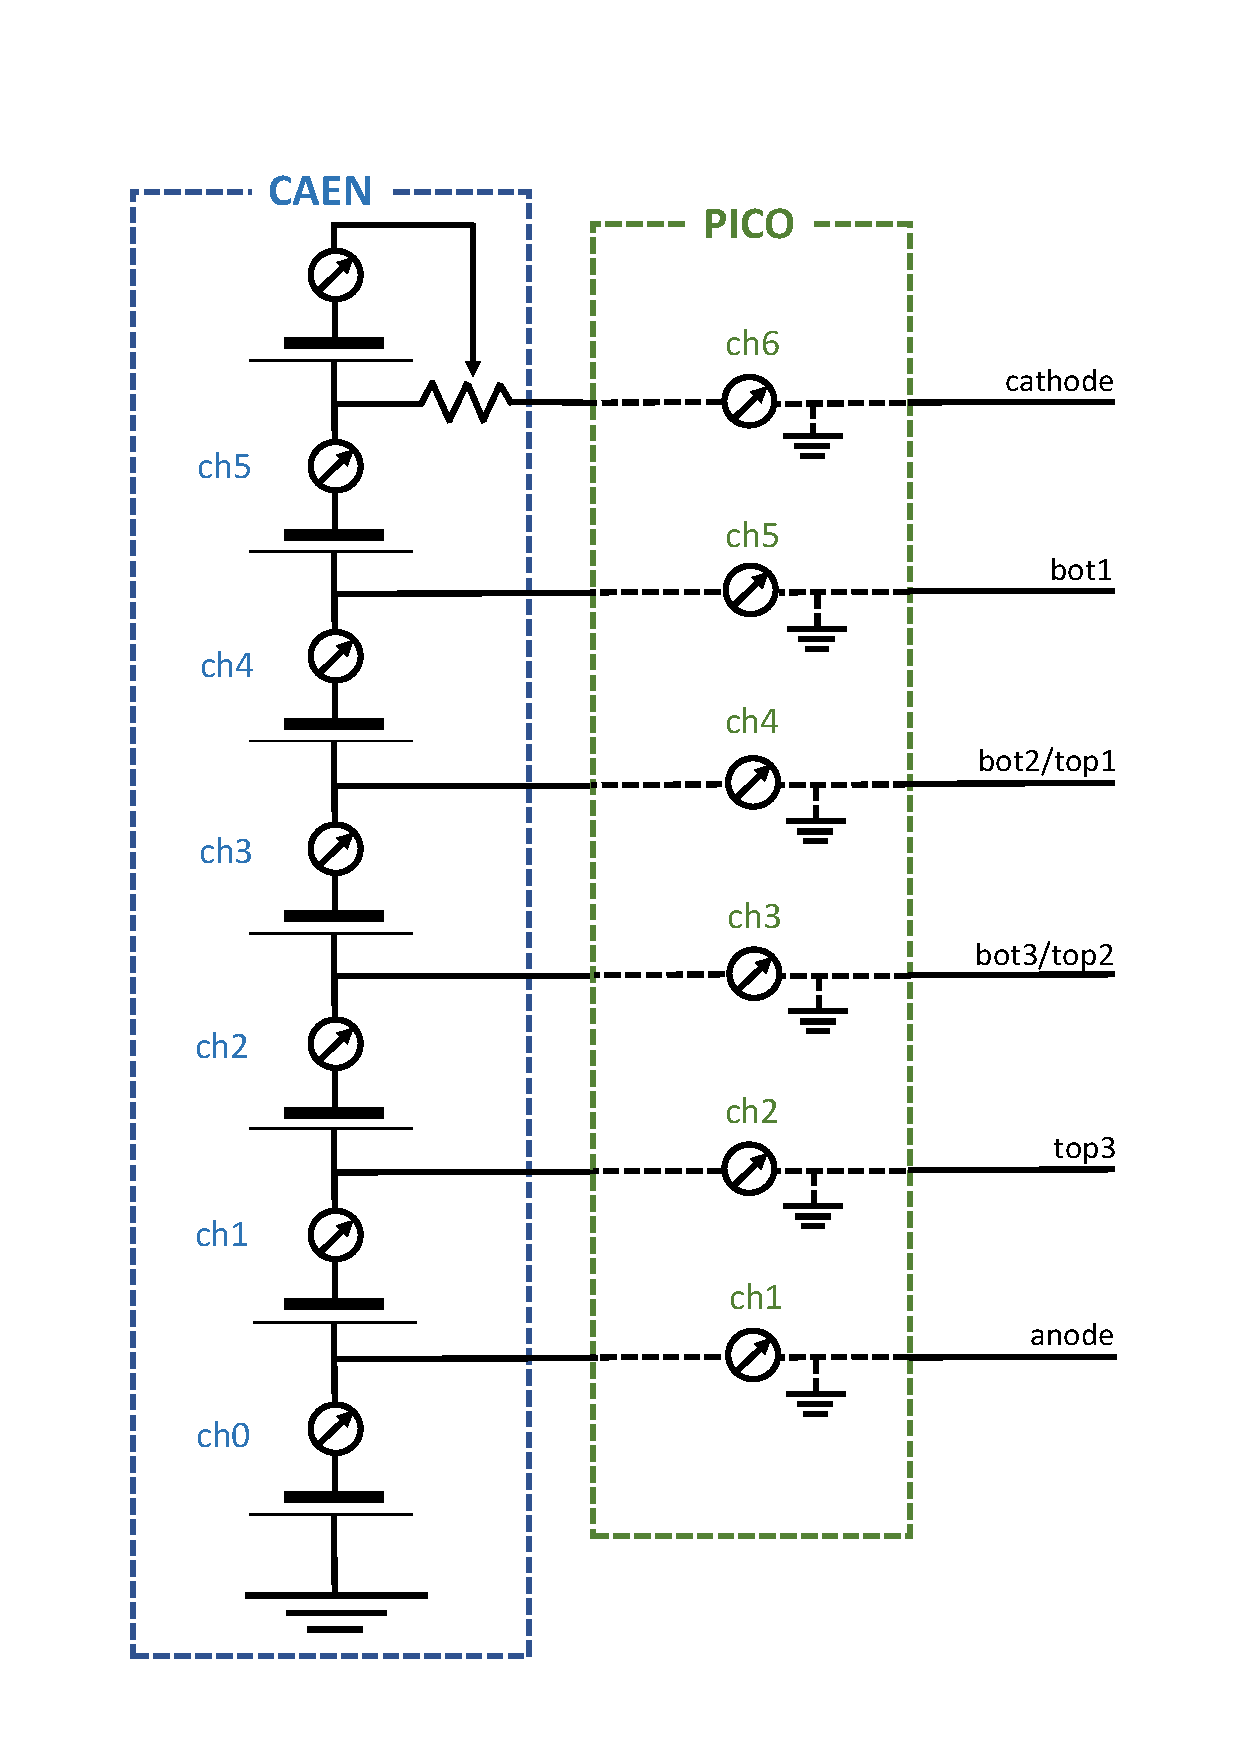
\includegraphics[width=0.8\textwidth]{Immagini/schema_canali.pdf}
	\caption{The channel scheme.}
	\label{fig:schema_canali}
\end{figure}

The gas chamber was filled with isobutane ($\mbox{C}_4\mbox{H}_{10}$) and its flow was of 145~sscm. 
The tests were performed at three different pressure: 10, 20 and 30~mbar. 



%parliamo di CAEN e PICO (non in maniera troppo approfondita)


%diagramma sui canali della lettura della corrente

inserire il plot run190 in cui si vede la misura fatta con PICO e quella con CAEN (per tutti e sei i canali!!)

%larghezza delle thgem � 107per107 mm2 e ci sono 143 file di buchi -> 20,000 buchi

%gas isobutano

%flow 145 sccm (standard cubic centimeter per minute)


range asimmetrico del bottom1, che ha minore precisione degli altri canali (farsi dire i valori da Alfonso)

\section{Method}





sorgente alpha e shutter, aprire e chiudere shutter, variazione di corrente

caratteristiche sorgente (55 kBq, 241Am)

rate di 140 Hz di particelle alpha

\section{Misure}

i canali 3 e 4 possono essere ignorati perch� non danno mai segnale

spieghiamo i diversi scan (induzione, thgem e drift)


\subsection{FULL THGEM}

partiamo dalle full thgem:

sulla parte di induzione: uno dei grafici con i quattro canali e la somma appropriata, 
incrocio fra corrente anodo e top3, regione di quasi plateau, poi la corrente aumenta, se avremo delle simulazione potremo corredare il discorso; obiettivo: cercare la regione di migliore funzionamento che dovrebbe essere quella del plateau



sulla parte delle thgem: andamento esponenziale, si raggiunge il limite di scarica, non sappiamo se la scarica � nelle thgem



sulla parte di drift: variare la corrente tra catodo e bottom1; a 0 volt abbiamo una misura: o lo strumento segna zero ma non � zerp 



descrizione delle varie pressioni: un grafico tenendo soltanto anodo a diverse pressioni, questo grafico non varia drammaticamente al variare della pressione; un altro grafico con l'induzione al variare della tensione delle thgem e/o del drift.



ion backflow: calcolare direttamente il valore in percentuale; unico grafico al variare delle pressioni; esso non dipende molto dall'induzione; esso dipende anche delle thgem (configurazione delle linee di forza); conclusione: 

fattore di moltiplicazione: inizialmente solo con le thgem piene;
poi thgem row e mostrare i tre grafici esemplari
induzione delle row thgem a 20 mbar � pi� bello;

\subsection{ROW THGEM}

la drift � da discutere: la loro geometria � diversa: 5 fila isolate e proviamo a spiegare che a basse tensioni della drift, il campo elettrico delle thgem forma un imbuto pi� largo, se vdrift aumenta la regione da cui le thgem raccolgono carica diminuisce

dalle row thgem ci aspettiamo meno corrente perch� hanno meno buchi: invece di 143 file, ne hanno 5, quindi hanno il 3.5\% dei buchi rispetto a quelle piene. In prima approssimazione potremmo aspettarci che il valore della corrente scali allo stesso modo. 

ion backflow nelle row � sistematicamente pi� alto; vediamo se l'andamento � simile; al variare dell'induzione diminuzione dell'IBF; 

%ricordarsi di fare la misura del drift delle row a 20 mbar
%ATTENZIONE: altri test tenendo i campi elettrici fissi
%Misura ad alta pressione con full thgem, misura ad altre pressione con row thgem e rifare i test cercando di mantenere i campi elettrici costanti (possibilmente con il drift a tensioni basse)



\section{Conclusioni}




\end{document}
